\chapter{Planning Documentation}
\label{chap:planning}

\section{Project Plan}
\label{sect:planning}

This section details the project timeline, task allocations and risk management strategies for the Cluedo/Clue! Desktop Game, developed in \texttt{\texttt{C\#}} / Unity.

\subsection{Initial Gantt Chart}
The initial project timeline and task assignments are visualised in the Gantt chart (Figure \ref{fig:gantt_chart}). This chart and the accompanying breakdown in Table \ref{tab:gantt_tasks} represent the final of the project schedule, serving as combination of every individual Gantt chart developed during each sprint.
\begin{figure}[H]
    \centering
    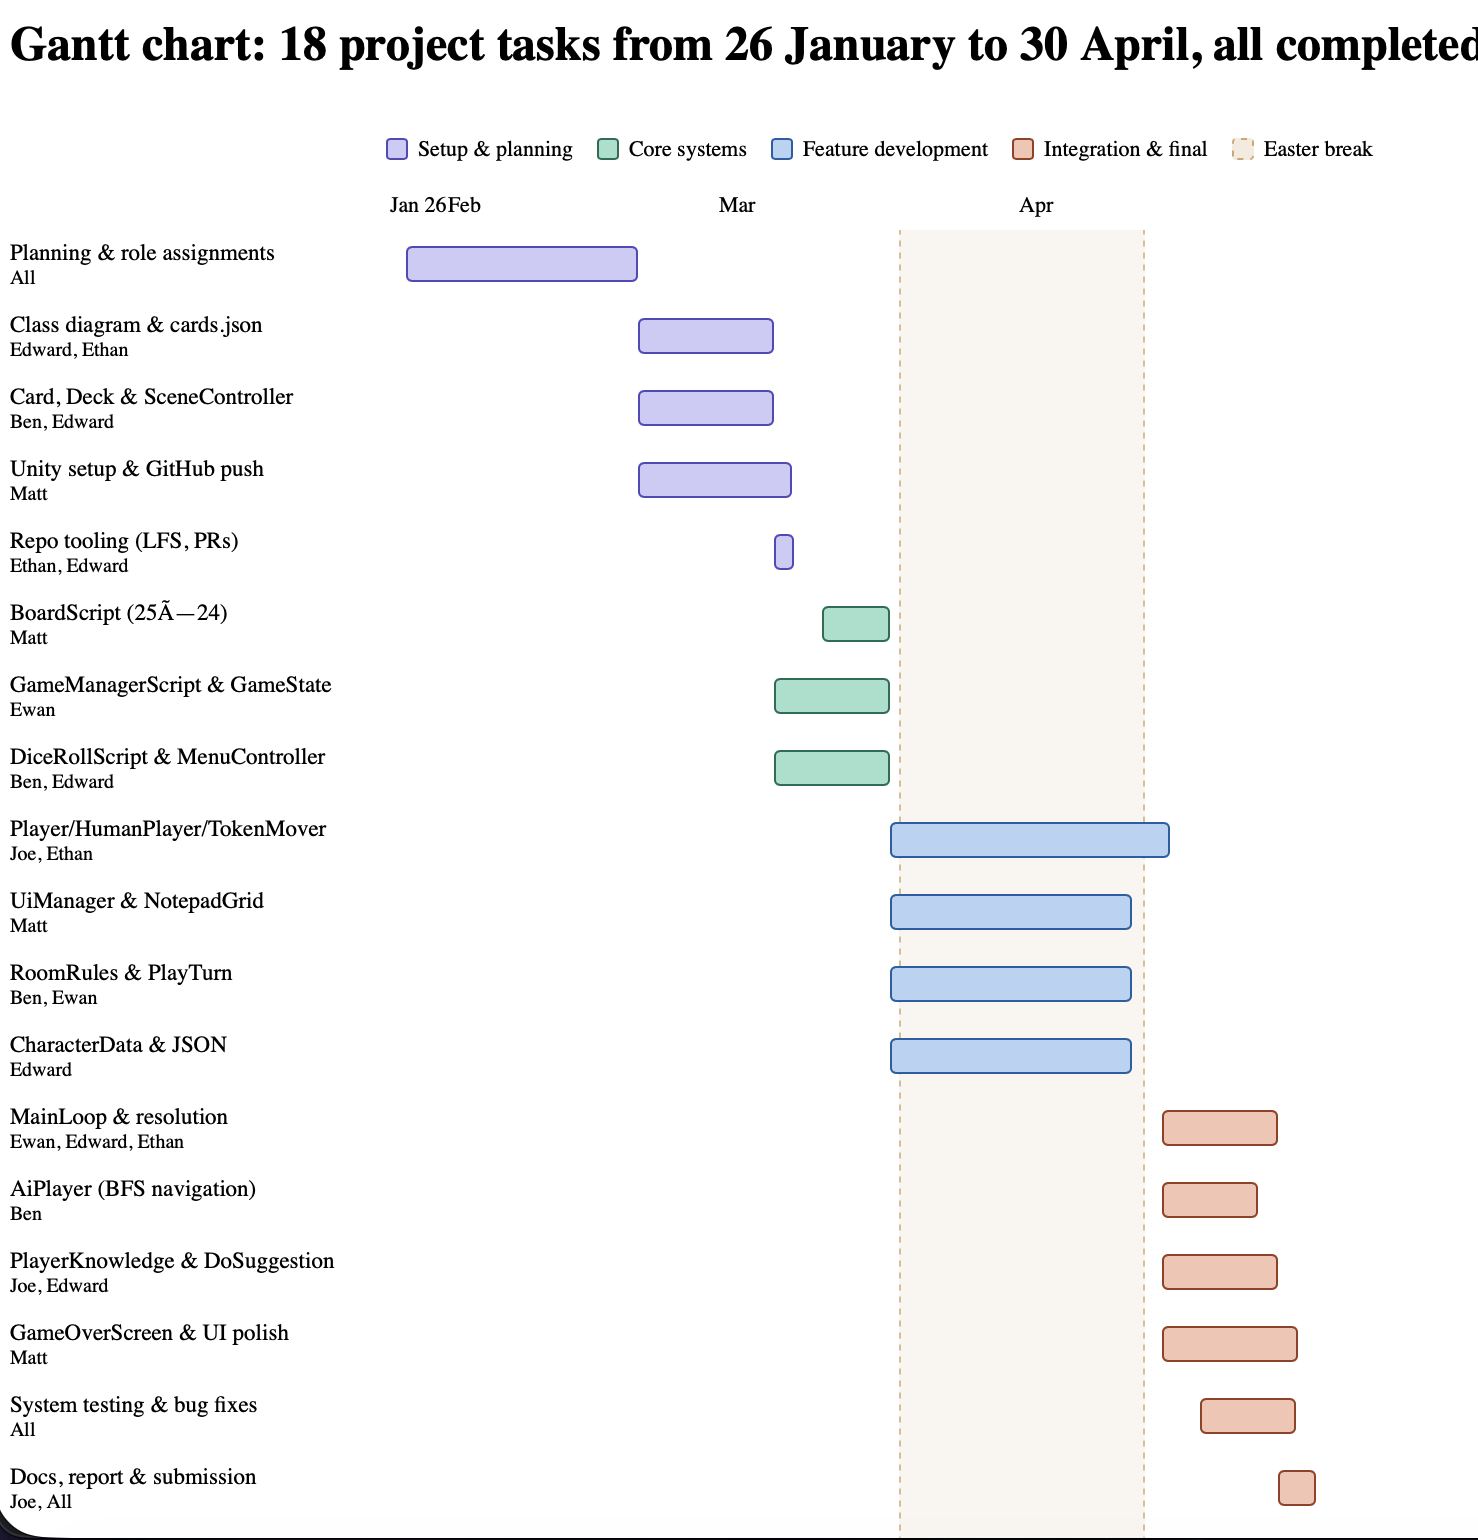
\includegraphics[width=\textwidth]{gantt.png}
    \caption{Unity project timeline (19 Feb -- 30 Apr 2026)}
    \label{fig:gantt_chart}
\end{figure}

\begin{table}[H]
    \centering
    \small
    \begin{tabular}{|p{6.2cm}|l|c|c|c|}
        \hline
        \textbf{Task} & \textbf{Owner(s)} & \textbf{Start} & \textbf{End} & \textbf{Status} \\ \hline
        Initial planning, meetings \& role assignments & All & 26 Jan & 19 Feb & Done \\ \hline
        Class diagram \& \texttt{cards.json} schema & Edward, Ethan & 19 Feb & 05 Mar & Done \\ \hline
        \texttt{Card}, \texttt{Deck} data classes \& \texttt{SceneController} & Ben, Edward & 19 Feb & 05 Mar & Done \\ \hline
        Unity project setup \& GitHub push & Matt & 19 Feb & 07 Mar & Done \\ \hline
        Repo tooling: Git LFS, PR templates, merge settings & Ethan, Edward & 05 Mar & 07 Mar & Done \\ \hline
        \texttt{BoardScript} (25$\times$24 tile array) & Matt & 10 Mar & 17 Mar & Done \\ \hline
        \texttt{GameManagerScript} singleton \& \texttt{GameState} & Ewan & 05 Mar & 17 Mar & Done \\ \hline
        \texttt{DiceRollScript} (physics) \& \texttt{MenuController} & Ben, Edward & 05 Mar & 17 Mar & Done \\ \hline
        \texttt{Player}/\texttt{HumanPlayer}/\texttt{TokenMover} (movement)$^*$ & Joe, Ethan & 17 Mar & 15 Apr & Done \\ \hline
        \texttt{UiManager}, \texttt{NotepadGrid} \& private modal & Matt & 17 Mar & 11 Apr & Done \\ \hline
        \texttt{RoomRules} (secret passages) \& \texttt{PlayTurn} coroutine & Ben, Ewan & 17 Mar & 11 Apr & Done \\ \hline
        \texttt{CharacterData} ScriptableObject \& JSON integration & Edward & 17 Mar & 11 Apr & Done \\ \hline
        \texttt{MainLoop}, suggestion \& accusation resolution & Ewan, Edward, Ethan & 14 Apr & 26 Apr & Done \\ \hline
        \texttt{AiPlayer} (BFS navigation, knowledge-filtered suggestions) & Ben & 14 Apr & 24 Apr & Done \\ \hline
        \texttt{PlayerKnowledge} \& \texttt{DoSuggestionThenAccusation} & Joe, Edward & 14 Apr & 26 Apr & Done \\ \hline
        \texttt{GameOverScreen} \& final UI polish & Matt & 14 Apr & 28 Apr & Done \\ \hline
        System testing, integration \& bug fixes & All & 18 Apr & 28 Apr & Done \\ \hline
        Documentation, report \& submission prep & Joe, All & 26 Apr & 30 Apr & Done \\ \hline
    \end{tabular}
    \caption{Final Consolidated Project Tasks and Timeline ($^*$Easter break 20~Mar -- 14~Apr: no development)}
    \label{tab:gantt_tasks}
\end{table}

\subsection{Critical Path}

The critical path runs through:

\begin{quote}
\textbf{BoardScript $\rightarrow$ GameManager $\rightarrow$ Deck/Cards $\rightarrow$ TokenMovement $\rightarrow$ GameLoop $\rightarrow$ Suggestion/Accusation $\rightarrow$ Win condition}
\end{quote}

Each task in this chain blocks the next: a player can only be \textit{placed} once the board exists; can only \textit{take a turn} once GameManager exists; can only \textit{move} once Deck/Cards is set up (the deck is built during game initialisation); can only \textit{make a Suggestion} once they are physically in a room (which requires TokenMovement); and can only \textit{win} via an Accusation evaluated against the solution envelope.

HandManager / CardInteraction sits on a \textit{parallel} branch off Deck/Cards --- Ben was able to develop the player hand UI during the same window as TokenMovement, so it does not appear on the critical path itself.

\subsubsection*{The Actual Bottleneck: TokenMovement}
TokenMovement was both the \textbf{longest single task} in the plan (17 Mar -- 15 Apr, $\sim$4 weeks) and the \textbf{task with the highest downstream impact} --- Suggestion, GameLoop progression, and AI movement all block on it. It was the right task to mark as the highest-risk item, and in practice it did slip slightly past its planned end date (see Revised Plan below).

\subsubsection*{Easter Break Disruption}
No development was scheduled or executed during the Easter holiday window (20 March -- 14 April). Effectively the critical path was paused for $\sim$3.5 weeks, which compressed Sprint 3 work into the second half of April and forced parallel execution of TokenMovement, GameLoop, and Suggestion in the final 10 days.

\subsection{Revised Plan}

The execution deviated from the initial Gantt in seven notable ways. They are recorded here so that a reader can compare the plan against what actually happened and understand why the team's structure changed during the project.

\begin{itemize}
    \item \textbf{Easter break paused development for $\sim$3.5 weeks:} There were \textbf{zero commits between 20 March and 14 April} on any branch. All the work nominally scheduled across the second half of Sprint 3 was compressed into the period 15--24 April.
    \item \textbf{TokenMovement slipped past its planned end date:} The major movement-fix commits actually landed on \textbf{17 April} and \textbf{18 April}. Legal-move detection on the irregular Cluedo board required more edge-case handling than the plan accounted for.
    \item \textbf{Suggestion / Accusation became a team task:} Originally assigned to Ewan, the work was distributed across Edward (guessing logic), Ethan (looping mechanisms), and Ewan (GameStateScript and menus) under time pressure.
    \item \textbf{Suggestion / Accusation logic merged into existing managers:} In the delivered codebase, the logic lives inside \texttt{GameManagerScript.cs} and \texttt{UiManager.cs} rather than in standalone classes. Splitting the classes cleanly would have required a refactor the team did not have time for (reflected in Chapter~\ref{chap:design-low}).
    \item \textbf{AI player scoped down:} The AI uses BFS-directed movement toward envelope-candidate rooms and knowledge-filtered suggestions; full notebook-based deduction (eliminating cards systematically) was not implemented (documented in Section~\ref{sec:sprint4}).
    \item \textbf{Sprint 2 absorbed unplanned repo infrastructure work:} Significant effort went into Git LFS setup, \texttt{.gitignore} fixes, PR templates, and Unity merge settings. This was necessary to prevent merge conflicts in Unity scenes but consumed feature development time.
    \item \textbf{Matt's script commits arrived late:} Matt's earlier work was contributed via pair-programming or was scene/asset work in Unity (which does not surface as distinct script commits). His first direct script commits in the repository arrived on 22--23 April.
\end{itemize}

\subsection{Effort Allocation}

Table \ref{tab:effort} shows the approximate hours per team member per sprint, estimated from Gantt task ownership, sprint-document contributions, and commit history. This justifies the peer-assessment split in Section~\ref{sec:peer-assessment}.

\begin{table}[H]
\centering
\caption{Effort Allocation (Approximate Hours)}
\label{tab:effort}
\begin{tabular}{|l|r|r|r|r|r|}
\hline
\textbf{Team Member} & \textbf{Sprint 1} & \textbf{Sprint 2} & \textbf{Sprint 3} & \textbf{Sprint 4} & \textbf{Total} \\ \hline
Edward & 8 & 12 & 14 & 18 & \textbf{52} \\ \hline
Ewan & 7 & 12 & 12 & 18 & \textbf{49} \\ \hline
Ethan & 8 & 9 & 14 & 14 & \textbf{45} \\ \hline
Joe & 7 & 8 & 14 & 16 & \textbf{45} \\ \hline
Ben & 5 & 9 & 11 & 14 & \textbf{39} \\ \hline
Matt & 6 & 9 & 10 & 15 & \textbf{40} \\ \hline
\textbf{Sprint Total} & \textbf{41} & \textbf{59} & \textbf{75} & \textbf{95} & \textbf{270} \\ \hline
\end{tabular}
\end{table}

\textit{Average 45 hours per person over the 10-week project (4.5 h/week).}
\subsection{Risk Analysis}

\subsubsection*{Risk Register}

\begin{table}[H]
\centering
\caption{Risk Register}
\label{tab:risk_register}
% This line forces the table to fit the text width
\resizebox{\textwidth}{!}{%
\begin{tabular}{|c|>{\centering\arraybackslash}p{4cm}|c|c|c|>{\centering\arraybackslash}p{4.5cm}|c|}
\hline
\textbf{ID} & \textbf{Risk} & \textbf{Likelihood} & \textbf{Impact} & \textbf{Severity} & \textbf{Mitigation Strategy} & \textbf{Owner} \\ \hline
R1 & Unity version incompatibility & 4 & 3 & High & Agree on LTS version; test in Sprint 1 & Matt \\ \hline
R2 & Git merge conflicts on scenes & 4 & 4 & High & Use UnityYAMLMerge; single owner per scene & Edward \\ \hline
R3 & Team member unable to contribute & 2 & 4 & Medium & Shared codebase knowledge; pair-coding & All \\ \hline
R4 & Scope creep & 3 & 3 & Medium & Prioritise core game loop first & Joe \\ \hline
R5 & Inconsistent physics dice & 3 & 2 & Medium & Fallback: default to 1 if result = 0 & Ben \\ \hline
R6 & AI player too complex & 3 & 2 & Low & Use random decision-making first & Ben \\ \hline
R7 & Corrupted submission file & 2 & 5 & Medium & Test zip unpacking before submission & Joe \\ \hline
R8 & Incomplete game loop & 2 & 5 & High & Prioritise end-to-end playable loop & All \\ \hline
R9 & Knowledge gap: Most of the team lacks prior experience with Unity or \texttt{C\#} & 5 & 4 & High & Allocate time in Sprint 1 for tutorials; pair-program with the experienced member & All \\ \hline
\end{tabular}%
} % Closes the resizebox
\end{table}

\subsubsection*{Risk Monitoring and Lessons Learned}

The team reviewed the risk register at the start of each sprint planning meeting.

\begin{itemize}
    \item \textbf{Sprint 1:} R1 was pre-empted. The team agreed on a Unity LTS version, and Edward seeded the repository with a working scene validated end-to-end. R9 materialised as the team's knowledge gap in Unity and C\# became apparent early on. To mitigate this, time was explicitly allocated in Sprint 1 for tutorials, and members relied heavily on pair-programming with the experienced team member to get up to speed.
    \item \textbf{Sprint 2:} R2 materialised (Unity scene merge conflicts) and R1 partially materialised (incomplete \texttt{.gitignore}). Ethan configured Git LFS, and Edward established Unity Smart Merge settings, PR compile-checks, and \texttt{.gitattributes} for \texttt{.unity} and \texttt{.prefab} files. The issue did not recur.
    \item \textbf{Sprint 3:} R3 materialised (the Easter break effectively paused all development for $\sim$3.5 weeks). R4 partially materialised as TokenMovement was more complex than estimated. The team scoped down TokenMovement, cutting A* pathfinding in favour of legal-move detection (documented in Section~\ref{sec:sprint3}).
    \item \textbf{Sprint 4:} R8 materialised (GameLoop, Suggestion, and AI were unfinished). R4 materialised via deliberate descoping under pressure. R2 re-emerged during the final integration push. Edward executed a large consolidate merge on 18 April. R7 was mitigated by verifying the zip unpacking before the deadline.
\end{itemize}

\textbf{Risks that did not materialise:}
R5 (physics dice fallback never triggered an invalid roll) and R6 (AI implementation was less difficult than expected, see section 2.4).

Lessons for Risk Planning:
\begin{enumerate}
    \item \textbf{Easter / holiday windows must be costed into the plan from the start.} Treating R3 as ``individual illness'' understated the systemic impact of a predictable shutdown.
    \item \textbf{Tool chain risks (R1, R2) have a higher early-impact than they appear.} Sprint 2 lost $\sim$1 week of feature work to repository tooling.
    \item \textbf{Scope-reduction is a valid mitigation.} Cutting some final UI tweaks preserved the critical path at the cost of design purity.
    \item \textbf{Account for learning curves in technical projects.} Identifying the knowledge gap (R9) early allowed the team to adjust Sprint 1 expectations, but future projects should formally budget time for upskilling.
\end{enumerate}

\newpage

% ==================== MEETING NOTES ====================
\section{Team Meetings}
\label{sect:meeting}

This section contains the records of all team meetings for the Clue! Simulation (G6046) project (Team 15: Ben, Edward, Ethan, Ewan, Joe, Matt). It details attendees, dates, summaries, agreed actions, and how risks were monitored and mitigated through decision-making.

\subsection{How to Read This Section}

\begin{quote}
The marking criterion for \textit{Planning -- meeting notes} (band 5) requires:
\textit{``A full set of notes that demonstrate an organised team, reflecting on progress on the project plan, and monitoring of risk factors identified, with appropriate mitigation through decision-making.''}

Each meeting below follows the same structure:
\begin{itemize}
    \item \textbf{Date / Duration / Attendees} --- for traceability and peer-assessment support.
    \item \textbf{Summary} --- what was discussed.
    \item \textbf{Decisions Made} --- outputs of the meeting (architectural, process, or planning).
    \item \textbf{Actions Agreed} --- owner-tagged tasks, each with a \textit{Completed?} column so the reader can see whether the action was actually delivered (band 4 requirement).
\end{itemize}

Cross-references: planning decisions feed the previous Project Plan section.
\end{quote}

\vspace{0.5cm}
\hrule
\vspace{0.5cm}

\subsection{Meeting 1}
\textbf{Date:} 26/01/2026 \\
\textbf{Duration:} $\sim$1 hour \\
\textbf{Attendees:} Ben, Edward, Ethan, Ewan, Joe, Matt

\subsubsection*{Summary}
\begin{itemize}
    \item Project briefing reviewed --- Watson Games' Cluedo simulation, desktop Mac/PC, with AI player and customisability requirements.
    \item Agreed to take a fluid approach to team roles --- tasks assigned based on who is best suited.
    \item Agreed to plan before deciding on a programming language.
    \item Began breaking down the classes that would be involved: Board, Players, Dice, Cards (Player, Room, Weapon), Grid of Judgements.
    \item Clarified the rules of the game.
    \item Agreed to use a statically typed language; discussed whether GUI should be 3D or 2D.
\end{itemize}

\subsubsection*{Decisions Made}
\begin{itemize}
    \item \textbf{Language/Platform:} Unity and \texttt{C\#} agreed upon (everyone in the group has little to no experience and would like to learn something new).
    \item \textbf{Frontend lead:} Matt.
    \item \textbf{Architecture:} Backend outputs a game state to the frontend, from which the frontend produces graphics.
    \item \textbf{Player branch:} One person to own the entire Player hierarchy (human and AI) to avoid confusion over inheritance.
    \item \textbf{Next meeting:} Monday the 1st.
\end{itemize}

\subsubsection*{Actions Agreed}
\begin{table}[H]
\centering
\resizebox{\textwidth}{!}{%
\begin{tabular}{|p{8cm}|l|l|}
\hline
\textbf{Action} & \textbf{Owner} & \textbf{Completed?} \\ \hline
Research Unity after meeting & All & Yes \\ \hline
Set up an empty Unity project as a ``spike'' to confirm everyone can run it & Edward & Yes --- initial commit 28/01 \\ \hline
Prepare for next meeting & All & Yes \\ \hline
\end{tabular}%
}
\end{table}

\vspace{0.5cm}
\hrule
\vspace{0.5cm}

\subsection{Meeting 2}
\textbf{Date:} 02/02/2026 \\
\textbf{Duration:} $\sim$1 hour 30 minutes \\
\textbf{Attendees:} Ben, Edward, Ethan, Ewan, Joe, Matt

\subsubsection*{Summary}
\begin{itemize}
    \item Reviewed Edward's Unity spike from the previous week --- confirmed the project compiles and runs on every team member's machine.
    \item Used the mark scheme to create a minimum viable plan, mapping out a full design plan and way of working.
    \item Agreed that the Board will be the main object in Unity --- parent to the majority of game parts.
    \item Agreed to make a skeleton code design of the entire game using a class diagram.
    \item Agreed to set up all specific documentation that the mark scheme mentions as we go through it.
    \item Agreed that after each commit to Git, each person is responsible for documenting what they have done.
    \item Agreed to create a schematic format for each commit to follow.
    \item Identified initial risks: Unity version drift between machines (R1) and Unity scene merge conflicts (R2) --- mitigations to be put in place before any feature work begins.
\end{itemize}

\subsubsection*{Decisions Made}
\begin{itemize}
    \item \textbf{Documentation:} Each person documents their own commits; a commit schematic format to be agreed and followed.
    \item \textbf{Design approach:} Class diagram to serve as the skeleton for the whole game.
    \item \textbf{Architecture:} Board as the main/parent object in Unity.
    \item \textbf{Risk register:} to be drafted formally and reviewed at every sprint planning meeting.
\end{itemize}

\subsubsection*{Actions Agreed}
\begin{table}[H]
\centering
\resizebox{\textwidth}{!}{%
\begin{tabular}{|p{8cm}|l|l|}
\hline
\textbf{Action} & \textbf{Owner} & \textbf{Completed?} \\ \hline
Create skeleton class diagram & Edward & Yes --- see \texttt{Design} docs \\ \hline
Agree commit schematic format & All & Yes --- followed across PRs \\ \hline
Set up documentation structure (\texttt{report/} folder) & Joe & Yes --- commits 19/02 \\ \hline
Draft initial risk register & Joe / Edward & Yes --- Table~\ref{tab:risk_register} \\ \hline
Continue building out basic Unity project structure & Edward & Yes --- commits 01/02 \\ \hline
\end{tabular}%
}
\end{table}

\vspace{0.5cm}
\hrule
\vspace{0.5cm}

\subsection{Meeting 3}
\textbf{Date:} 19/02/2026 \\
\textbf{Duration:} 1 hour 45 minutes \\
\textbf{Attendees:} Ben, Edward, Ethan, Ewan, Joe \textit{(Matt absent)}

\subsubsection*{Summary}
\begin{itemize}
    \item Agreed to use a standard format template for every meeting going forward.
    \item Main discussion centred around class structure.
    \item Sprint role assignments were started and partially agreed.
    \item Important game logic realisations and discussions took place.
    \item Decided to use XML comments for code documentation.
    \item Agreed sprint plan working backwards from deadline.
\end{itemize}

\subsubsection*{Decisions Made}

\textbf{Code Documentation:} \texttt{C\#} XML doc comments agreed as the standard.

\textbf{Privacy model discussed:} Options considered: (A) pass-and-play single screen, (B) cards hidden/revealed on demand via private modal, (C) split screen. \textbf{Agreed: Option B} --- Matt to implement a private modal in \texttt{UiManager} so revealed cards are shown only to the suggesting player.

\textbf{Data-driven design:} Board layout, character names, weapon names loaded from JSON files using Unity's built-in JsonUtility.

\begin{table}[H]
\centering
\caption*{Role Assignments}
\resizebox{\textwidth}{!}{%
\begin{tabular}{|l|p{8cm}|l|}
\hline
\textbf{Area} & \textbf{Scope} & \textbf{Assigned To} \\ \hline
\textbf{Game Logic \& Rules} & GameManager, turn flow, suggestions, accusations, win conditions & Ewan \\ \hline
\textbf{Board \& Movement} & Board grid, rooms, doors, pathfinding, secret passages & Joe, Ethan \\ \hline
\textbf{Card System} & Cards, dealing, murder envelope & Ben \\ \hline
\textbf{UI / GUI} & Board rendering, player HUD, detective notepad, menus & Matt \\ \hline
\textbf{Data Handling} & Loading/saving from JSON, designed data structure & Edward \\ \hline
\textbf{Diagrams \& Plans} & Gantt chart (or similar), UML diagram & Joe \\ \hline
\textbf{AI Player Agent} & Random agent first, then improved strategy if time allows & Ben \\ \hline
\textbf{Testing \& Docs} & Test plans, unit tests, sprint docs, meeting notes, report & Everyone \\ \hline
\end{tabular}%
}
\end{table}

\begin{table}[H]
\centering
\caption*{Sprint Plan}
\resizebox{\textwidth}{!}{%
\begin{tabular}{|l|l|p{8cm}|}
\hline
\textbf{Sprint} & \textbf{Focus} & \textbf{Key Deliverables} \\ \hline
Sprint 1 & Core logic & Board representation, player movement, turn system, dice, cards \\ \hline
Sprint 2 & Core gameplay & Suggestions, accusations, UI card logic, detective notes, rooms \\ \hline
Sprint 3 & AI \& polish & Random AI player agent, GUI polish, JSON loading \\ \hline
Sprint 4 & Testing \& docs & System/unit testing, bug fixes, documentation, final integration \\ \hline
\end{tabular}%
}
\end{table}

\subsubsection*{Actions Agreed}
\begin{table}[H]
\centering
\resizebox{\textwidth}{!}{%
\begin{tabular}{|p{6cm}|l|l|l|}
\hline
\textbf{Action} & \textbf{Owner} & \textbf{Due} & \textbf{Completed?} \\ \hline
Set up Unity project in GitHub repo & Matt & Next meeting & Yes (07 Mar) \\ \hline
Create shared documentation folder & Joe & Next meeting & Yes (19/02) \\ \hline
Write up retrospective notes for 1 \& 2 & Joe & Next meeting & Yes (19/02) \\ \hline
Draft initial Gantt chart / project plan & Joe & Next meeting & Yes \\ \hline
Design board data file schema (JSON) & Edward & --- & Yes \\ \hline
Create initial class diagram & Edward, Ethan & --- & Yes \\ \hline
Begin Sprint 1 work on assigned area & All & --- & Yes \\ \hline
\end{tabular}%
}
\end{table}

\vspace{0.5cm}
\hrule
\vspace{0.5cm}

\subsection{Meeting 4}
\textbf{Date:} 05/03/2026 \\
\textbf{Duration:} $\sim$1 hour \\
\textbf{Attendees:} Ben, Edward, Ethan, Ewan, Joe, Matt

\subsubsection*{Summary}
\begin{itemize}
    \item \textbf{Sprint 1 close.} Reviewed deliverables: Deck and Card classes, JSON schema, basic Unity scene with placeholder board.
    \item Discussion on whether sprint roles need to change for Sprint 2. Agreed the \textit{Tiles and Board} role is no longer a separate area; absorbed into Matt's UI ownership.
    \item Reviewed risks. R1 (Unity version) had not materialised. R2 (merge conflicts) flagged as the next likely risk now that real feature work was about to begin in parallel.
    \item Agreed Sprint 2 priorities: BoardScript, GameManagerScript singleton, DiceRollScript with physics, token spawning, repo clean-up / Git LFS.
    \item Brief retrospective: documentation kept up; commit schematic being followed inconsistently --- agreed to enforce more strictly via the PR template.
\end{itemize}

\subsubsection*{Decisions Made}
\begin{itemize}
    \item \textbf{Role change:} Tiles and Board role removed as a separate area; responsibilities absorbed into UI (Matt).
    \item \textbf{Sprint 1 closed.} All Sprint 1 objectives met.
    \item \textbf{Sprint 2 plan:} Core gameplay infrastructure. Repo tooling (Git LFS, \texttt{.gitattributes}, PR templates) to be set up \textit{before} any feature work to mitigate R2.
    \item \textbf{PR-template enforcement:} Edward to add a ``large PR'' warning workflow and a Unity compile-check workflow on PRs.
\end{itemize}

\subsubsection*{Actions Agreed}
\begin{table}[H]
\centering
\resizebox{\textwidth}{!}{%
\begin{tabular}{|p{6cm}|l|l|l|}
\hline
\textbf{Action} & \textbf{Owner} & \textbf{Due} & \textbf{Completed?} \\ \hline
Set up Git LFS and clean up the repo & Ethan & Before Sp 2 & Yes (06/03) \\ \hline
Add PR templates, compile checks & Edward & Before Sp 2 & Yes (07/03) \\ \hline
Add Unity smart merge settings & Edward & Before Sp 2 & Yes (07/03) \\ \hline
Begin \texttt{BoardScript} (25$\times$24 tile encoding) & Matt & Sprint 2 & Yes (10/03) \\ \hline
Begin \texttt{GameManagerScript} (setup) & Ewan & Sprint 2 & Yes \\ \hline
Begin \texttt{DiceRollScript} (Rigidbody) & Ben & Sprint 2 & Yes \\ \hline
Refine class diagram alongside dev & Edward, Ethan & Ongoing & Yes \\ \hline
\end{tabular}%
}
\end{table}

\vspace{0.5cm}
\hrule
\vspace{0.5cm}

\subsection{Meeting 5}
\textbf{Date:} 10/03/2026 \\
\textbf{Duration:} $\sim$1 hour 30 minutes \\
\textbf{Attendees:} Ben, Edward, Ethan, Ewan, Joe, Matt

\subsubsection*{Summary}
\begin{itemize}
    \item Mid-Sprint-2 check-in. Repo tooling from Meeting 4 had landed --- confirmed merge conflicts no longer breaking the build.
    \item Detailed discussion on the division of backend work and Matt's frontend. Agreed \texttt{GameManagerScript} is the bridge; UI scripts should never read the board state directly.
    \item Matt walked the team through the Unity editor, scene hierarchy, and \texttt{MonoBehaviour} lifecycle methods. Important for backend-focused members.
    \item Edward flagged that the current \texttt{DeckScript} was blocking progress on \texttt{GameManagerScript}. Agreed Edward would lead a Deck refactor.
    \item Discussed turn-order --- agreed to hardcode standard Cluedo order for simplicity.
\end{itemize}

\subsubsection*{Decisions Made}
\begin{itemize}
    \item \textbf{Backend / frontend boundary:} \texttt{GameManagerScript} is the single bridge. Matt's UI consumes its API.
    \item \textbf{Customisation:} Character names, weapons, room names loaded from \texttt{cards.json}. Adding/changing a card requires only a JSON edit.
    \item \textbf{Deck refactor:} Edward to refactor \texttt{DeckScript} so it initialises cleanly from GameManager.
    \item \textbf{Turn order:} Hardcoded as Miss Scarlett $\rightarrow$ Mustard $\rightarrow$ White $\rightarrow$ Green $\rightarrow$ Peacock $\rightarrow$ Plum.
\end{itemize}

\subsubsection*{Actions Agreed}
\begin{table}[H]
\centering
\resizebox{\textwidth}{!}{%
\begin{tabular}{|p{8cm}|l|l|}
\hline
\textbf{Action} & \textbf{Owner} & \textbf{Completed?} \\ \hline
Refactor \texttt{DeckScript} so it initialises from GameManager & Edward & Yes (11/03) \\ \hline
Continue \texttt{GameManagerScript} (singleton + setup) & Ewan & Yes (17/03) \\ \hline
Begin token spawning logic in \texttt{GameManagerScript} & Edward & Yes (17/03) \\ \hline
Flesh out \texttt{PlayerScripts} (player state container) & Joe & Yes (17/03) \\ \hline
Finalise \texttt{Card} / \texttt{Deck} data classes & Ben & Yes (17/03) \\ \hline
Confirm \texttt{cards.json} covers 6 chars, 6 weapons, 9 rooms & Edward & Yes \\ \hline
\end{tabular}%
}
\end{table}

\vspace{0.5cm}
\hrule
\vspace{0.5cm}

\subsection{Meeting 6}
\textbf{Date:} 17/03/2026 \\
\textbf{Duration:} $\sim$1 hour \\
\textbf{Attendees:} Ben, Edward, Ethan, Ewan, Joe, Matt

\subsubsection*{Summary}
\begin{itemize}
    \item Sprint 2 review --- board, game manager, dice and token spawning working.
    \item Decision made to formalise a \texttt{GameState} singleton to manage Playing/MainMenu/GameOver instead of handling it ad hoc.
    \item Reviewed role assignments --- board/tiles work largely complete so Joe and Ethan to shift focus to \texttt{TokenMovementScript}.
    \item Discussed how to handle turn sequence --- Ewan to own the main loop.
    \item Edward to look into how \texttt{SceneController} persists data.
\end{itemize}

\subsubsection*{Decisions Made}
\begin{itemize}
    \item \textbf{GameState singleton} to manage game-wide state transitions.
    \item \textbf{SceneController} to use \texttt{DontDestroyOnLoad} to persist player counts.
    \item Board/tile work considered done; Joe and Ethan move to movement.
\end{itemize}

\subsubsection*{Actions Agreed}
\begin{table}[H]
\centering
\resizebox{\textwidth}{!}{%
\begin{tabular}{|p{8cm}|l|l|}
\hline
\textbf{Action} & \textbf{Owner} & \textbf{Completed?} \\ \hline
Implement \texttt{GameState} & Ewan & Yes \\ \hline
Begin \texttt{TokenMovementScript} & Joe, Ethan & Yes \\ \hline
Integrate \texttt{DiceRollScript} result into turn start & Ben & Yes \\ \hline
Finalise \texttt{SceneController} with DontDestroyOnLoad & Edward & Yes \\ \hline
Begin \texttt{MenuController} scene transition & Edward & Yes \\ \hline
\end{tabular}%
}
\end{table}

\vspace{0.5cm}
\hrule
\vspace{0.5cm}

\subsection{Meeting 7}
\textbf{Date:} 31/03/2026 \\
\textbf{Duration:} $\sim$1 hour 15 minutes \\
\textbf{Attendees:} Ben, Edward, Ethan, Ewan, Joe, Matt

\subsubsection*{Summary}
\begin{itemize}
    \item Sprint 3 progress review --- token movement working for basic corridor navigation.
    \item Identified issue: two competing implementations in \texttt{TokenMovementScript} (int array vs Vector2Int). Agreed to keep Vector2Int.
    \item Discussed card reveal during suggestions --- Matt to handle private modal.
    \item Room entry needs mapping door tile values (2--11) to strings.
    \item Discussed AI --- agreed random legal moves are sufficient.
\end{itemize}

\subsubsection*{Decisions Made}
\begin{itemize}
    \item \textbf{\texttt{Vector2Int}} adopted as standard; old \texttt{int[]} movement approach removed.
    \item \textbf{\texttt{UiManager}} to be the single point of contact for all player-facing UI.
    \item \textbf{Room mapping} to map door IDs 2--11 to room names.
    \item \textbf{AI movement:} random selection from \texttt{GetLegalMoves()} --- no A* pathfinding.
\end{itemize}

\subsubsection*{Actions Agreed}
\begin{table}[H]
\centering
\resizebox{\textwidth}{!}{%
\begin{tabular}{|p{8cm}|l|l|}
\hline
\textbf{Action} & \textbf{Owner} & \textbf{Completed?} \\ \hline
Clean up \texttt{TokenMovementScript} --- remove old \texttt{int[]} & Joe & Yes \\ \hline
Implement \texttt{TokenMover.EnterRoom()} \& string mapping & Ben & Yes \\ \hline
Complete \texttt{UiManager} prompts and private modal & Matt & Yes \\ \hline
Implement \texttt{NotepadGrid} toggle UI & Matt & Yes \\ \hline
Wire AI random move into \texttt{PlayTurn} coroutine & Ewan, Joe & Yes \\ \hline
Everyone write up own contribution notes & All & Partially (in Sp 4) \\ \hline
\end{tabular}%
}
\end{table}

\vspace{0.5cm}
\hrule
\vspace{0.5cm}

\subsection{Meeting 8}
\textbf{Date:} 14/04/2026 \\
\textbf{Duration:} $\sim$1 hour \\
\textbf{Attendees:} Ben, Edward, Ethan, Ewan, Joe \textit{(Matt absent)}

\subsubsection*{Summary}
\begin{itemize}
    \item Sprint 3 close --- prototype playable to the point of entering rooms.
    \item Ewan identified suggestion \textit{resolution} (clockwise card-showing) as the most complex remaining piece; top priority for Sprint 4.
    \item Noted \texttt{MenuController} hardcoded counts --- logged as known issue.
    \item Ben to complete AI suggestion generation.
    \item \texttt{GameOverScreen} needed for end state.
    \item Submission deadline reminder: 30 April, 4PM.
\end{itemize}

\subsubsection*{Decisions Made}
\begin{itemize}
    \item \textbf{Sprint 4 priority:} (1) Suggestion resolution, (2) Accusation, (3) AI suggestions, (4) Game over screen, (5) Docs.
    \item \textbf{Known issues logged:} Hardcoded menu counts and spawn issues with $<$ 6 players will be documented rather than delaying Sprint 4 logic.
\end{itemize}

\subsubsection*{Actions Agreed}
\begin{table}[H]
\centering
\resizebox{\textwidth}{!}{%
\begin{tabular}{|p{8cm}|l|l|}
\hline
\textbf{Action} & \textbf{Owner} & \textbf{Completed?} \\ \hline
Implement \texttt{ResolveSuggestion()} clockwise coroutine & Ewan & In progress \\ \hline
Implement accusation check vs \texttt{GetEnvelope()} & Ewan & In progress \\ \hline
AI random suggestion when in room & Ben & In progress \\ \hline
\texttt{GameOverScreen} --- restart and return-to-menu & Matt & Yes \\ \hline
Fill sprint docs and report skeleton & Joe, All & In progress \\ \hline
Record any known bugs for testing documentation & All & In progress \\ \hline
\end{tabular}%
}
\end{table}

\vspace{0.5cm}
\hrule
\vspace{0.5cm}

\subsection{Meeting 9}
\textbf{Date:} 20/04/2026 \\
\textbf{Duration:} $\sim$45 minutes \\
\textbf{Attendees:} Ben, Edward, Ethan, Ewan, Joe \textit{(Matt absent)}

\subsubsection*{Summary}
\begin{itemize}
    \item Sprint 4 mid-point check-in. Ewan demoed suggestion resolution working end-to-end.
    \item Accusation logic implemented. Incorrect accusation eliminates player.
    \item AI player takes full turns (rolls, moves, enters rooms, suggests).
    \item \texttt{GameOverScreen} wired up and working.
    \item Discussed peer assessment and final submission logistics.
\end{itemize}

\subsubsection*{Decisions Made}
\begin{itemize}
    \item Accusation to be offered as an option after a suggestion is resolved, not as a separate mandatory step.
    \item Known issues formally documented rather than attempting a last-minute fix.
    \item Final submission ZIP to be verified by group before uploading.
\end{itemize}

\subsubsection*{Actions Agreed}
\begin{table}[H]
\centering
\resizebox{\textwidth}{!}{%
\begin{tabular}{|p{8cm}|l|l|}
\hline
\textbf{Action} & \textbf{Owner} & \textbf{Completed?} \\ \hline
Wire accusation UI option after suggestion resolution & Ewan & In progress \\ \hline
Fix / document $<$ 6 player token spawn issue & Ethan & In progress \\ \hline
Fill all sprint doc test result columns & All & In progress \\ \hline
Complete group report (achievements, lessons) & Joe & In progress \\ \hline
Agree peer assessment marks & All & Before 30 Apr \\ \hline
Record gameplay video (MP4) & Matt & Before 29 Apr \\ \hline
Final submission ZIP upload to Canvas & TBC & By 30 Apr 4PM \\ \hline
\end{tabular}%
}
\end{table}

\newpage
